\documentclass[tikz,border=10pt]{standalone}
\usepackage{tikz}
\usetikzlibrary{shapes.geometric, arrows.meta, positioning, fit, backgrounds, calc}

\begin{document}
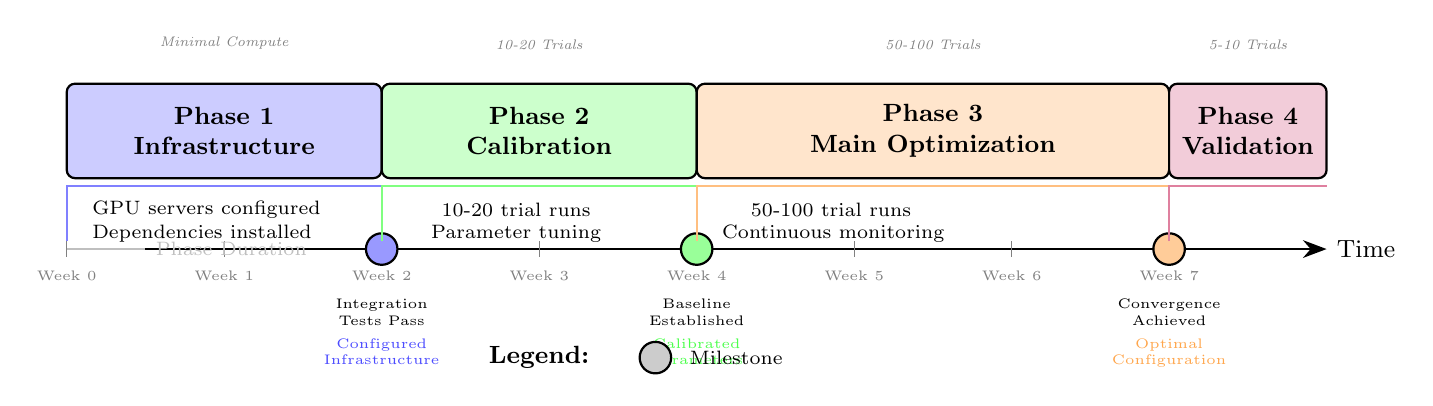
\begin{tikzpicture}[
    node distance=0.3cm,
    phase/.style={rectangle, draw=black, thick, minimum height=1.2cm, align=center, rounded corners=3pt, font=\small\bfseries},
    milestone/.style={circle, draw=black, thick, fill=white, minimum size=0.4cm, inner sep=0pt},
    task/.style={rectangle, draw=none, minimum width=3cm, minimum height=0.5cm, align=left, font=\scriptsize},
    arrow/.style={-{Stealth[length=2.5mm]}, thick}
]

% Timeline base
\draw[thick, -{Stealth[length=3mm]}] (0,0) -- (16,0) node[right, font=\small] {Time};

% Week markers
\foreach \x/\week in {0/0, 2/1, 4/2, 6/3, 8/4, 10/5, 12/6, 14/7} {
    \draw[gray] (\x,-0.1) -- (\x,0.1);
    \node[below, font=\tiny, gray] at (\x,-0.15) {Week \week};
}

% Phase 1: Infrastructure Setup (Weeks 0-2)
\node[phase, fill=blue!20, minimum width=4cm] at (2,1.5) (p1) {Phase 1\\Infrastructure};
\draw[thick, blue!50] (0,0.1) -- (0,0.8) -- (4,0.8) -- (4,0.1);

% Phase 1 milestones
\node[milestone, fill=blue!40] at (4,0) (m1) {};
\node[below=0.3cm of m1, font=\tiny, align=center] {Integration\\Tests Pass};

% Phase 1 tasks
\node[task, anchor=west] at (0.2,0.5) {GPU servers configured};
\node[task, anchor=west] at (0.2,0.2) {Dependencies installed};

% Phase 2: Calibration (Weeks 2-4)
\node[phase, fill=green!20, minimum width=4cm] at (6,1.5) (p2) {Phase 2\\Calibration};
\draw[thick, green!50] (4,0.1) -- (4,0.8) -- (8,0.8) -- (8,0.1);

% Phase 2 milestones
\node[milestone, fill=green!40] at (8,0) (m2) {};
\node[below=0.3cm of m2, font=\tiny, align=center] {Baseline\\Established};

% Phase 2 tasks
\node[task, anchor=west] at (4.2,0.5) {10-20 trial runs};
\node[task, anchor=west] at (4.2,0.2) {Parameter tuning};

% Phase 3: Main Optimization (Weeks 4-8)
\node[phase, fill=orange!20, minimum width=6cm] at (11,1.5) (p3) {Phase 3\\Main Optimization};
\draw[thick, orange!50] (8,0.1) -- (8,0.8) -- (14,0.8) -- (14,0.1);

% Phase 3 milestones
\node[milestone, fill=orange!40] at (14,0) (m3) {};
\node[below=0.3cm of m3, font=\tiny, align=center] {Convergence\\Achieved};

% Phase 3 tasks
\node[task, anchor=west] at (8.2,0.5) {50-100 trial runs};
\node[task, anchor=west] at (8.2,0.2) {Continuous monitoring};

% Phase 4: Validation (Weeks 8-10, shown partially)
\node[phase, fill=purple!20, minimum width=2cm] at (15,1.5) (p4) {Phase 4\\Validation};
\draw[thick, purple!50] (14,0.1) -- (14,0.8) -- (16,0.8);

% Compute budget indicators
\node[above=0.3cm of p1, font=\tiny\itshape, color=gray] {Minimal Compute};
\node[above=0.3cm of p2, font=\tiny\itshape, color=gray] {10-20 Trials};
\node[above=0.3cm of p3, font=\tiny\itshape, color=gray] {50-100 Trials};
\node[above=0.3cm of p4, font=\tiny\itshape, color=gray] {5-10 Trials};

% Deliverables below timeline
\node[below=0.8cm of m1, font=\tiny, align=center, text width=2cm, color=blue!70] {Configured\\Infrastructure};
\node[below=0.8cm of m2, font=\tiny, align=center, text width=2cm, color=green!70] {Calibrated\\Parameters};
\node[below=0.8cm of m3, font=\tiny, align=center, text width=2cm, color=orange!70] {Optimal\\Configuration};

% Legend
\node[below=2cm of p2, font=\small\bfseries] (legend) {Legend:};
\node[milestone, fill=gray!40, right=0.5cm of legend] (legmile) {};
\node[right=0.1cm of legmile, font=\scriptsize] {Milestone};
\draw[thick, gray!50, right=1.5cm of legmile] (0,0) -- (1,0) node[right, font=\scriptsize] {Phase Duration};

\end{tikzpicture}
\end{document}
